\documentclass[a4paper,10pt]{article}
\usepackage[utf8]{inputenc}
\usepackage{graphicx}
\usepackage{gensymb}
\usepackage{textcomp}

%opening
\title{
  \begin{large}
    Signals \& Systems
    Assignment No. 6
  \end{large}
}
\author{P.Anurag\\ 17MCME13}

\begin{document}

\maketitle
\section{ write down as a difference equation with non-linearity; take a and c as 5 digit prime numbers and plot output for 1000 values.}
  \begin{figure}[!hbt]
    \centering
      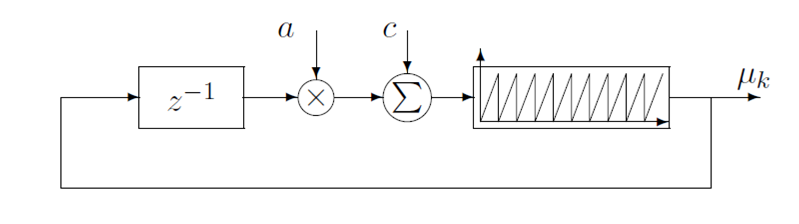
\includegraphics[scale=0.65]{image002.png}
    \caption{Linear congrential generator}
  \end{figure}

  \Large{Sol:- }
  The non-linear function in the above block diagram is modulo.
\end{document}
